\chapter{State of the art chess engines}
\label{chap:ch3}

\section{Top Chess Engine Championship}
\label{sec:ch3sec1}

The Top Chess Engine Championship (TCEC) is internationally recognized as one of the most prestigious and competitive computer chess tournaments in the world.

TCEC is an online tournament that features the strongest chess engines competing in a round-robin format (each engine plays in turn against every other engine), followed by knockout stages to determine the champion. The engines compete on powerful hardware, and each match consists of multiple games with different time controls and openings to ensure a diverse range of positions and scenarios.

TCEC has been held several times a year since 2010, and 24 seasons have concluded as of May 2023. Stockfish holds the record of being a 14-time winner of the TCEC. Stockfish and Leela Chess Zero have dominated the competition in the past years, with the final having been played between the two engines in 9 of the last 11 seasons.

\section{Elo rating system}
\label{sec:ch3sec2}

The Elo rating system is a technique used to determine the comparative levels of skill among players in games with zero-sum outcomes. FIDE (Fédération Internationale des Échecs), the international governing body for chess, embraced the Elo rating system in 1970 and continues to employ it as the primary method for evaluating player skill to this present day.

A player's Elo rating is denoted by a numerical value that might increase or decrease based on the outcomes of the rated games they play.

Elo's rating system operates on the premise that every player possesses an unknown current playing ability, which is approximated by a rating. When players with (unknown) strengths $R_A$ and $R_B$ engage in a game, the projected score for player A is assumed to be

\begin{equation}
    E=\frac{1}{1+10^{-(R_A-R_B)/400}},
\end{equation}

where the score corresponds to 1 in the event of player A's victory, $1/2$ in case of a draw, and 0 if player A loses \cite{glickman1999rating}.

Following each match, the victorious player subtracts rating points from their defeated opponent, with the total points gained or lost being determined by the disparity in their ratings. If the player with a higher rating wins, only a small number of rating points are deducted from the lower-rated player. Conversely, if the lower-rated player achieves an unexpected victory, a substantial number of rating points is transferred from the higher-rated player to the lower-rated player.

When a game results in a draw, the lower-rated player receives a small number of points from the higher-rated player. Therefore, this rating system possesses a self-correcting mechanism. Players whose ratings are either too low or too high will eventually outperform or underperform, respectively, compared to the expectations set by the rating system. Consequently, these players will gain or lose rating points until their ratings align with their true playing ability.

Elo ratings are solely comparative and hold validity only within the specific rating pool in which they were computed, rather than serving as an absolute measure of a player's proficiency. The highest Elo rating attained by a human was 2882, accomplished by Magnus Carlsen in May 2014 on the FIDE ratings list \cite{fide-ratings-May2014}. It is estimated that top chess engines possess over 3400 Elo points.

\section{Stockfish}
\label{sec:ch3sec3}

The strongest chess engine is currently Stockfish, an open-source project. It uses a minimax algorithm to search for the most promising positions, along with alpha-beta pruning, iterative deepening, and other improvements to reduce the search-space \cite{maharaj2022chess}. For evaluating the positions, Stockfish uses a hand-crafted evaluation function that consists of multiple features: material, position of the pieces on the board, structure of the pawns, mobility of pieces, safety of the king etc. \cite{lai2015giraffe}

Recent versions of Stockfish have been improved with NNUE (Efficiently Updatable Neural Networks). NNUE is a neural network-based evaluation function. Unlike traditional evaluation functions that are based on handcrafted features and heuristics, NNUE evaluates a chess position by analyzing it directly with a neural network. Because the neural network can learn and improve its evaluation of positions over time through training, the evaluation function becomes more flexible and adaptable.

Stockfish uses a multi-layer neural network architecture that receives a representation of the present board state as input and generates a score that reflects the anticipated outcome of the game. The neural network is trained using a dataset of high-quality chess games, where the inputs are positions from the games and the outputs are the eventual outcomes of the games.

NNUE has been a significant development in computer chess, as it has led to significant improvements in the playing strength of the Stockfish engine. In particular, NNUE has improved Stockfish's ability to evaluate endgame positions, which were previously challenging for traditional evaluation functions to handle.

\section{AlphaZero}
\label{sec:ch3sec4}

AlphaZero is an engine first published in 2017 by Google division Deepmind. It mastered the board games of chess, shogi and go, comprehending them exclusively through the rules and without any additional game-specific human knowledge or data.

AlphaZero uses Monte Carlo Tree Search instead of the minimax approach. This algorithm does not need an evaluation function, since it can compute meaningful evaluations based on random playouts that reach terminal game states, where the win/draw/loss outcome can be applied. Still, combining it with a strong evaluation function helps improve it.

DeepMind, the team behind the engine, built an evaluation function through deep reinforcement learning, training it with the matches the engine played itself. This brings the advantage that there is no need for hand-crafted feature selection and no data, since it generates the data by itself, and, with enough training, the model can learn its own useful features.

Another advantage of the Monte Carlo Tree Search algorithm is that the performance is expected to gradually grow with the computation time and the number of iterations. Iterative deepening in minimax can provide some resemblance to this behavior, but it is typically less "smooth" because the method takes far longer each time the depth is raised than it did for the previous depth. If it runs out of time, it must abandon the current search at the current depth limit; the last search will be useless, and the results from the previous search will be used instead.

AlphaZero was trained for 9 hours in chess, and reached Stockfish's level in the first 4 hours of training. AlphaZero was tested by the DeepMind team against Stockfish 8. In 1000 games, it won 155, lost only 6, and drew the other 839. AlphaZero played some additional matches starting from common human openings, and it managed to defeat Stockfish in all of them, "suggesting that AlphaZero has mastered a wide spectrum of chess play" \cite{silver2018general}.

Stockfish 8 is estimated to have around 3400 Elo points, while AlphaZero's playing strength would correspond to an Elo of over 3400 (fig. \ref{fig:alphaZeroEloEvolution}).

\begin{figure}[h]
    \centering
    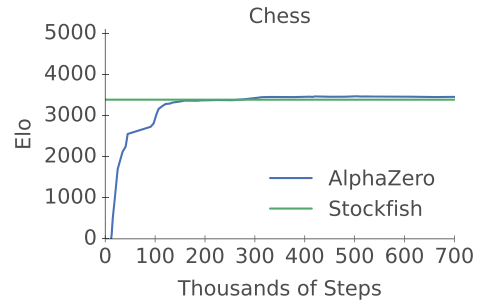
\includegraphics[width=0.6\textwidth]{figures/alpha-zero-elo-evolution.png}
    \caption{AlphaZero Elo evolution over training steps \cite{silver2018general}}
    \label{fig:alphaZeroEloEvolution}
\end{figure}

\section{Leela Chess Zero}
\label{sec:ch3sec5}

Leela Chess Zero (LCZero) is a computer chess engine based on the principles of DeepMind's AlphaZero. Since AlphaZero is not open-source, and there was no way to test the results stated in DeepMind's paper, LCZero was created by a group of developers led by Gary Linscott, who started the project in 2018. The engine was largely driven by the community of chess enthusiasts and programmers, who contributed to the project by providing computing resources.

LCZero developers also brought some key improvements to the AlphaZero approach:
\begin{itemize}
    \item Efficient implementation: LCZero is designed to run efficiently on standard hardware, such as CPUs and GPUs commonly available to consumers. This makes it more accessible than AlphaZero, which was trained on specialized hardware
    \item Improved neural network architecture: LCZero's neural network architecture is optimized for the game of chess, with modifications that allow it to better represent the game state and learn from self-play. This has led to better performance in practice. The developers also added Squeeze and Excitation (SE) layers to the neural network, which improve the representation of CNNs (Convolutional Neural Networks), by enabling them to selectively attend to the most important features of the input data
    \item Dynamic evaluation: LCZero uses a dynamic evaluation function during self-play, which allows it to better evaluate the value of positions and guide its search. Unlike AlphaZero, which uses a fixed evaluation function throughout the self-play process, LCZero updates its evaluation function after each game played, based on the results and the positions encountered. This allows it to adapt to changes in the playing style and strategy of its opponents
\end{itemize}

In April 2018, LCZero became the first engine to join the TCEC that used a deep neural network. At first, it didn't perform well, but by September 2018, it achieved a level of competitive performance comparable to the strongest chess engines in the world, and in 2019 and 2020 it won the competition. Since joining the TCEC, LCZero has achieved significant success, having won the competition twice, secured the second place on seven occasions, and achieved third place once.

On its official website \cite{lczero-training}, LCZero is currently rated over 3500 Elo points (fig. \ref{fig:leelaChessZeroEloEvolution}).

\begin{figure}[h]
    \centering
    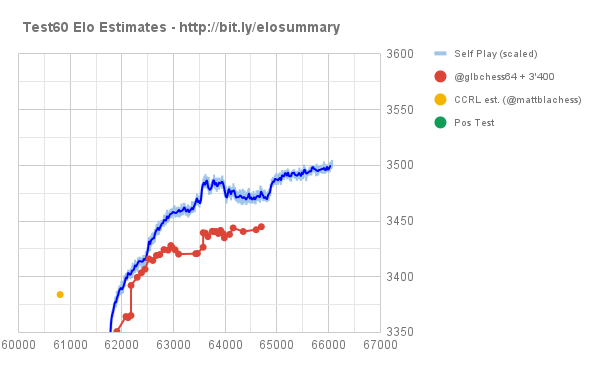
\includegraphics[width=0.9\textwidth]{figures/leela-chess-zero-elo-evolution.png}
    \caption{Leela Chess Zero Elo evolution by different metrics \cite{lczero-training}}
    \label{fig:leelaChessZeroEloEvolution}
\end{figure}